%!TEX root=masterproef.tex

\subsection{Opbouw}

Figuur \ref{fig:devel-component-overview} geeft een overzicht van de opbouw van
de oplossing.

\begin{figure}[ht]
  \centering
  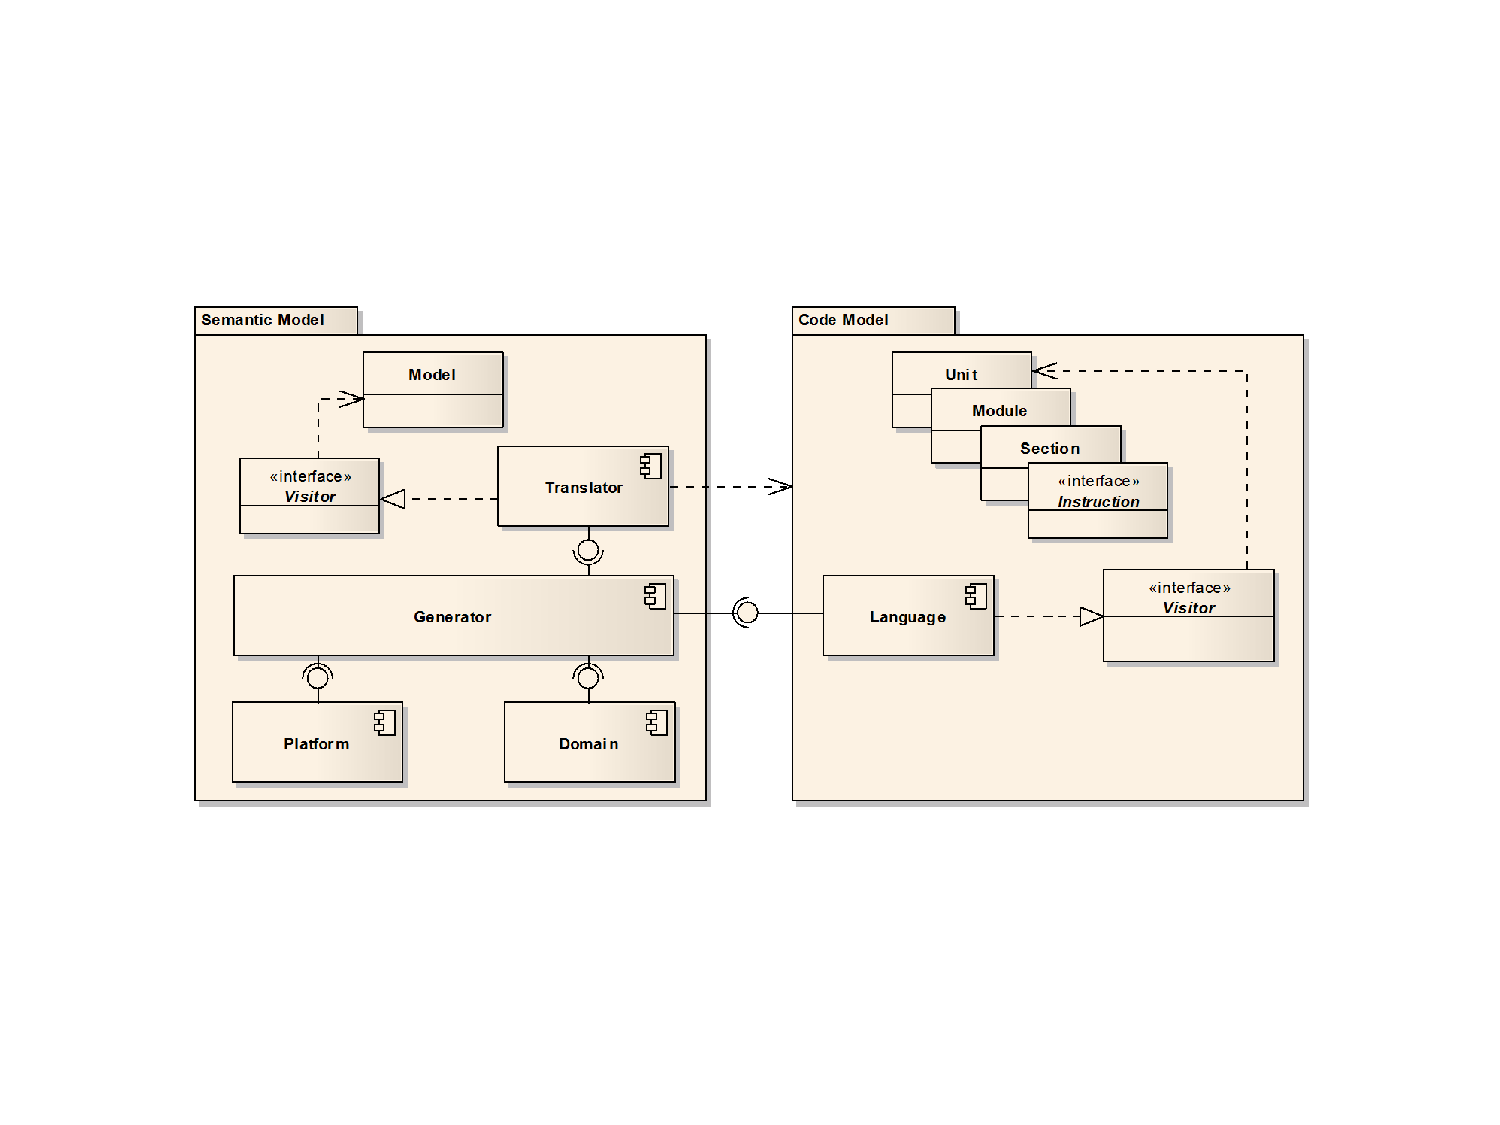
\includegraphics[width=\linewidth]{resources/component-overview.pdf}
  \caption{Overzicht van componenten en kernentiteiten}
  \label{fig:devel-component-overview}
\end{figure}

Intern bestaat de oplossing uit twee grote delen: het semantische en het
code-gedeelte. Binnen het semantische gedeelte vinden we het SM terug. Dit
model kan benaderd worden door middel van een zgn. \emph{visitor}, een
implementatie van het \emph{visitor}-patroon. Aan de hand van deze
\emph{visitor} kunnen transformaties van het model gerealiseerd worden.

Het SM is de primaire invoer voor de generator. Deze kan zijn taak slechts
vervullen door middel van een compositie met een \emph{platform-} en
\emph{domeinindefinitie}, een vertaler (\emph{Translator}) die elementen uit
het semantische gedeelte kan omzetten naar overeenkomstige elementen in het
code-gedeelte, en de uiteindelijk beoogde programmeertaal (\emph{Language}).

De programmeertaal maakt deel uit van het code-gedeelte, wat in hoofdzaak het
CM bevat. Dit is op zijn beurt opgebouwd uit een hi\"erarchie van vier niveaus.
De structuur van de beoogde code wordt weergegeven door de compilatie
\emph{unit}, de \emph{modules} en de \emph{secties}. Hier staat de unit voor
het geheel, de modules voor functioneel samenhangende delen en de secties voor
een fysieke opdeling in bestanden. De juiste realisatie van deze hi\"erarchie
wordt overgelaten aan de implementatie van de taal die hier betekenis aan kan
geven.

Op het laagste niveau van het CM vinden we de \emph{instructies}. Deze kunnen
gebruikt worden om effectieve code voor te stellen. Er bestaat in het CM per
definitie een overeenkomstige instructie voor elk element uit het SM. Aangezien
het SM functioneel rijker is dan de meeste programmeertalen, moeten na
constructie van het initi\"ele CM, door middel van transformaties,
alternatieven ge\"implementeerd worden, die binnen de mogelijkheden van de
uiteindelijke programmeertaal liggen.

\subsection{ANTLR}
\label{subsection:devel-antlr}

Het generatieproces start met het inladen van de FOO-lang-bronbestanden in het
SM. Dit gebeurt door middel van een \emph{parser} die de tekstuele voorstelling
analyseert en de semantische constructies detecteert. Het resultaat van deze
stap is een boomstructuur die de betekenis van de verschillende constructies
structureel weergeeft. Zo'n boomstructuur is een AST. Figuur
\ref{fig:devel-ast} toont de AST van het elementaire voorbeeld uit
codevoorbeeld \ref{lst:hello.foo}.

\begin{figure}[ht]
  \centering
  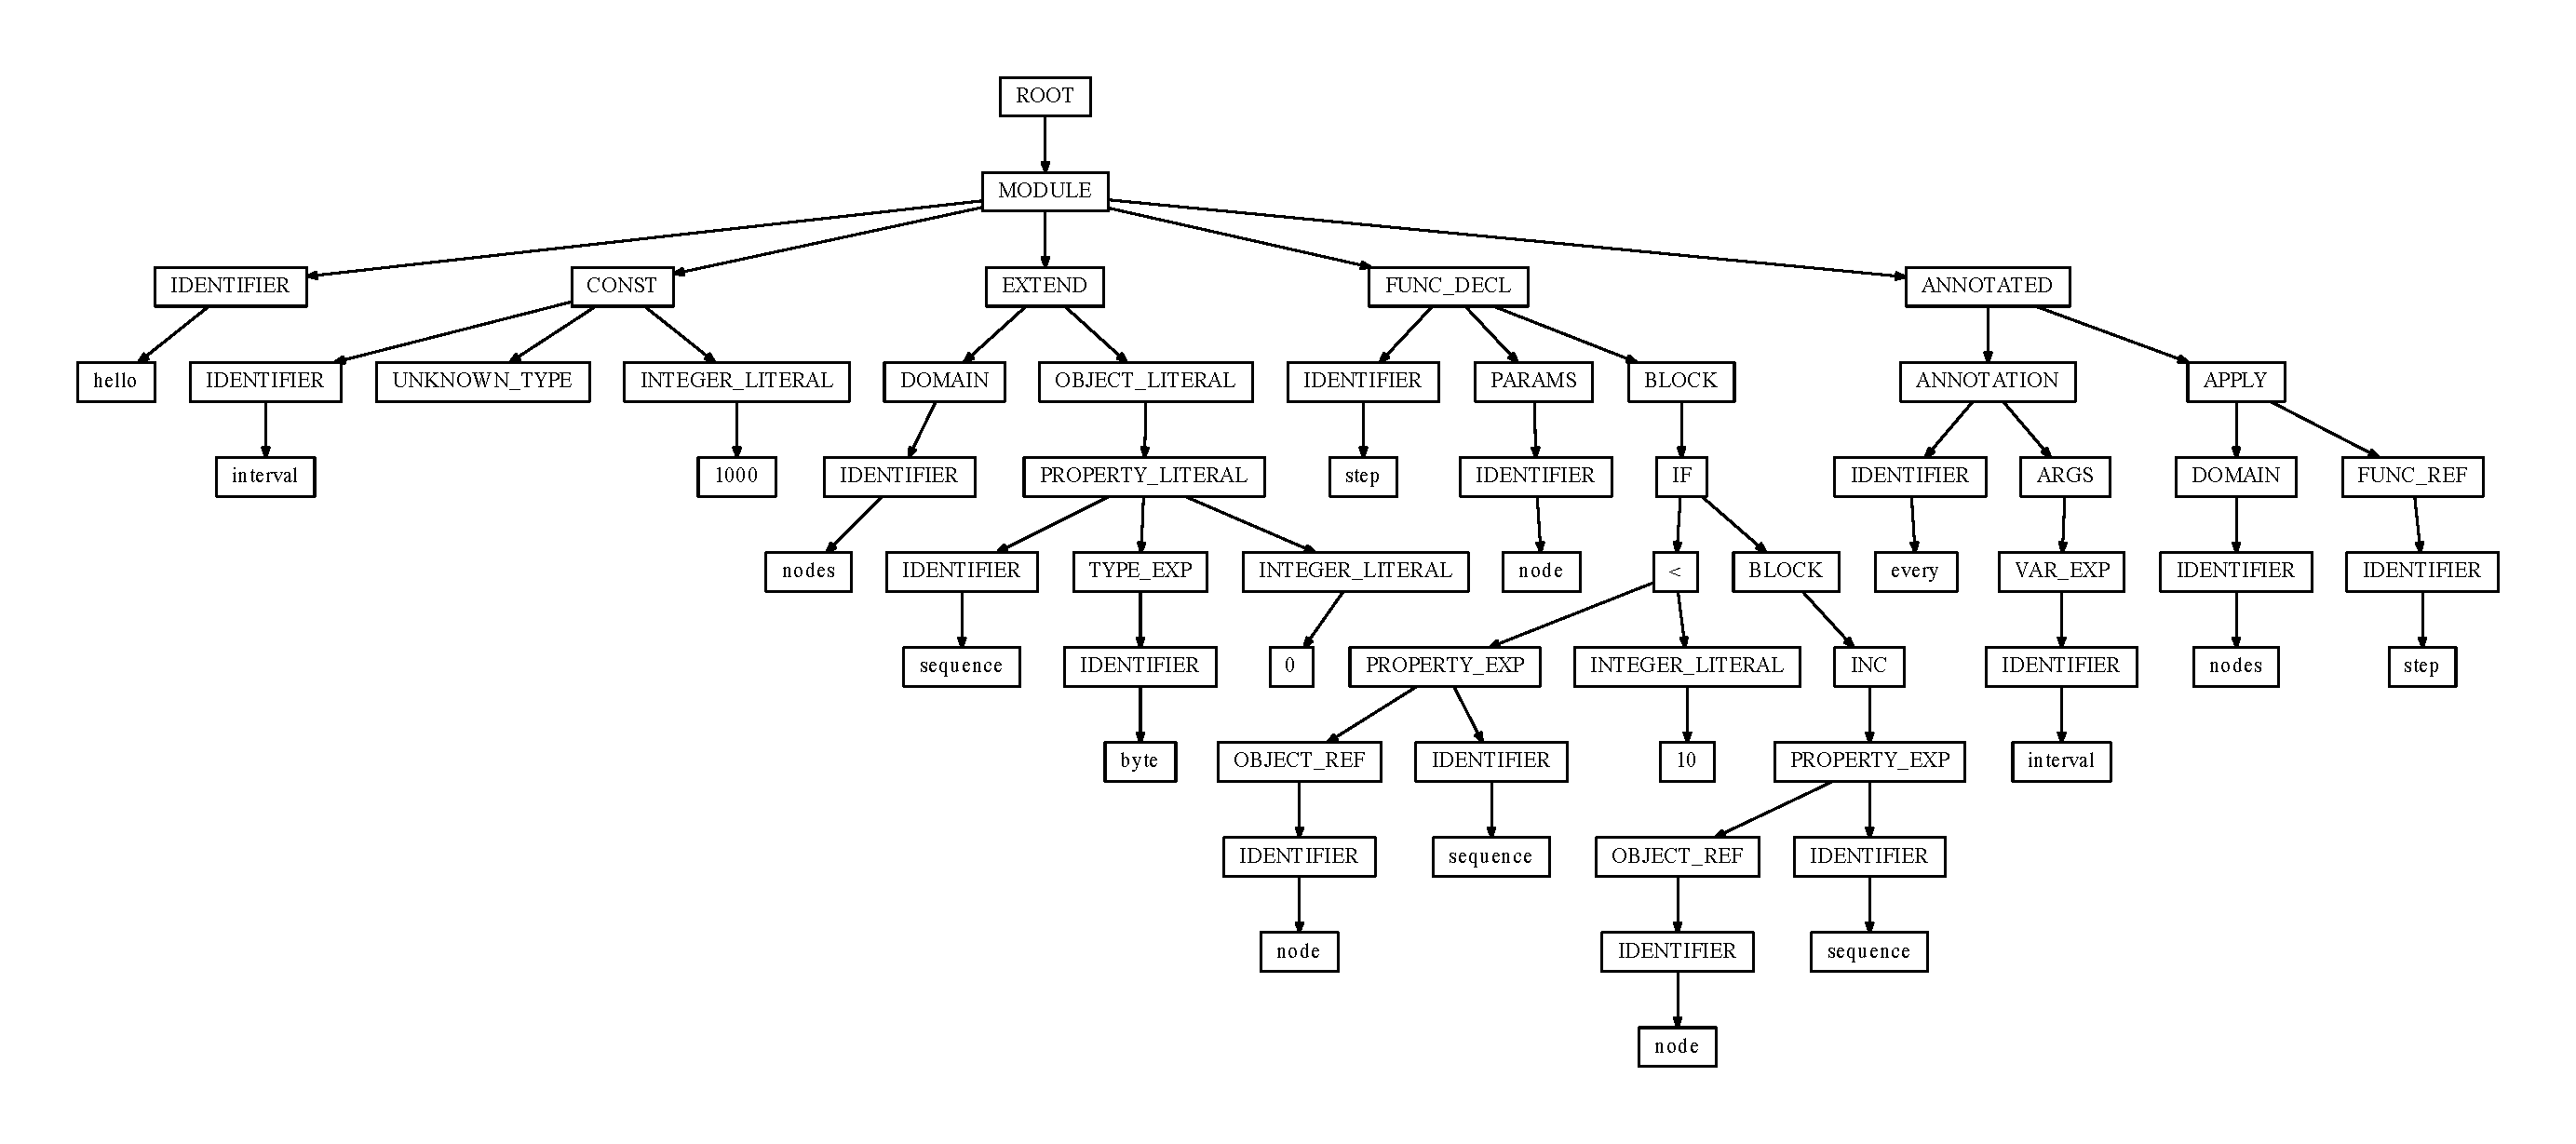
\includegraphics[width=\linewidth]{resources/hello_ast.pdf}
  \caption{De AST van het elementaire voorbeeld, \ttt{hello.foo}}
  \label{fig:devel-ast}
\end{figure}

We herkennen de inhoud van het codevoorbeeld in deze figuur: op het hoogste
niveau zien we de module met een naam (\ttt{IDENTIFIER}), de definitie van een
constante (\ttt{CONST}), een uitbreiding van het domein (\ttt{EXTEND}), een
functiedefinitie (\ttt{FUNC\_DECL}) en een geannoteerde applicatie
(\ttt{ANNOTATED}) van een functie op een domein. De AST is ontdaan van alle
ondersteunende syntax, zoals aanduidingen voor blokken code\dots en bevat
louter de semantische inhoud.
